\label{ch:datasets}

Deep learning is a fundamentally data-driven approach. It aims to progressivly optimize a complicated model by minimizing its loss over a large variety of training inputs; therefore these inputs are of crucial importance when trying to obtain a certain desired behaviour. They must be organized and relevant to the task, and each input, which in our case is an image, must be associated with a ground truth, which encodes the ideal result that the network should strive for. Errors or inaccuracies in the ground truth or the inputs introduce noise that could greatly influence the final results.

This chapter will examine the process that brought to the creation of the datasets used to train our model. It will start by examining LINEMOD\cite{linemod}, a commonly used dataset for 6D pose estimation, and then cover the iterations and reasoning behind the choices that led to the creation of our own custom dataset.

\section{The LINEMOD Dataset}
\label{s:LINEMOD}

\begin{figure}[h]
    \centering
    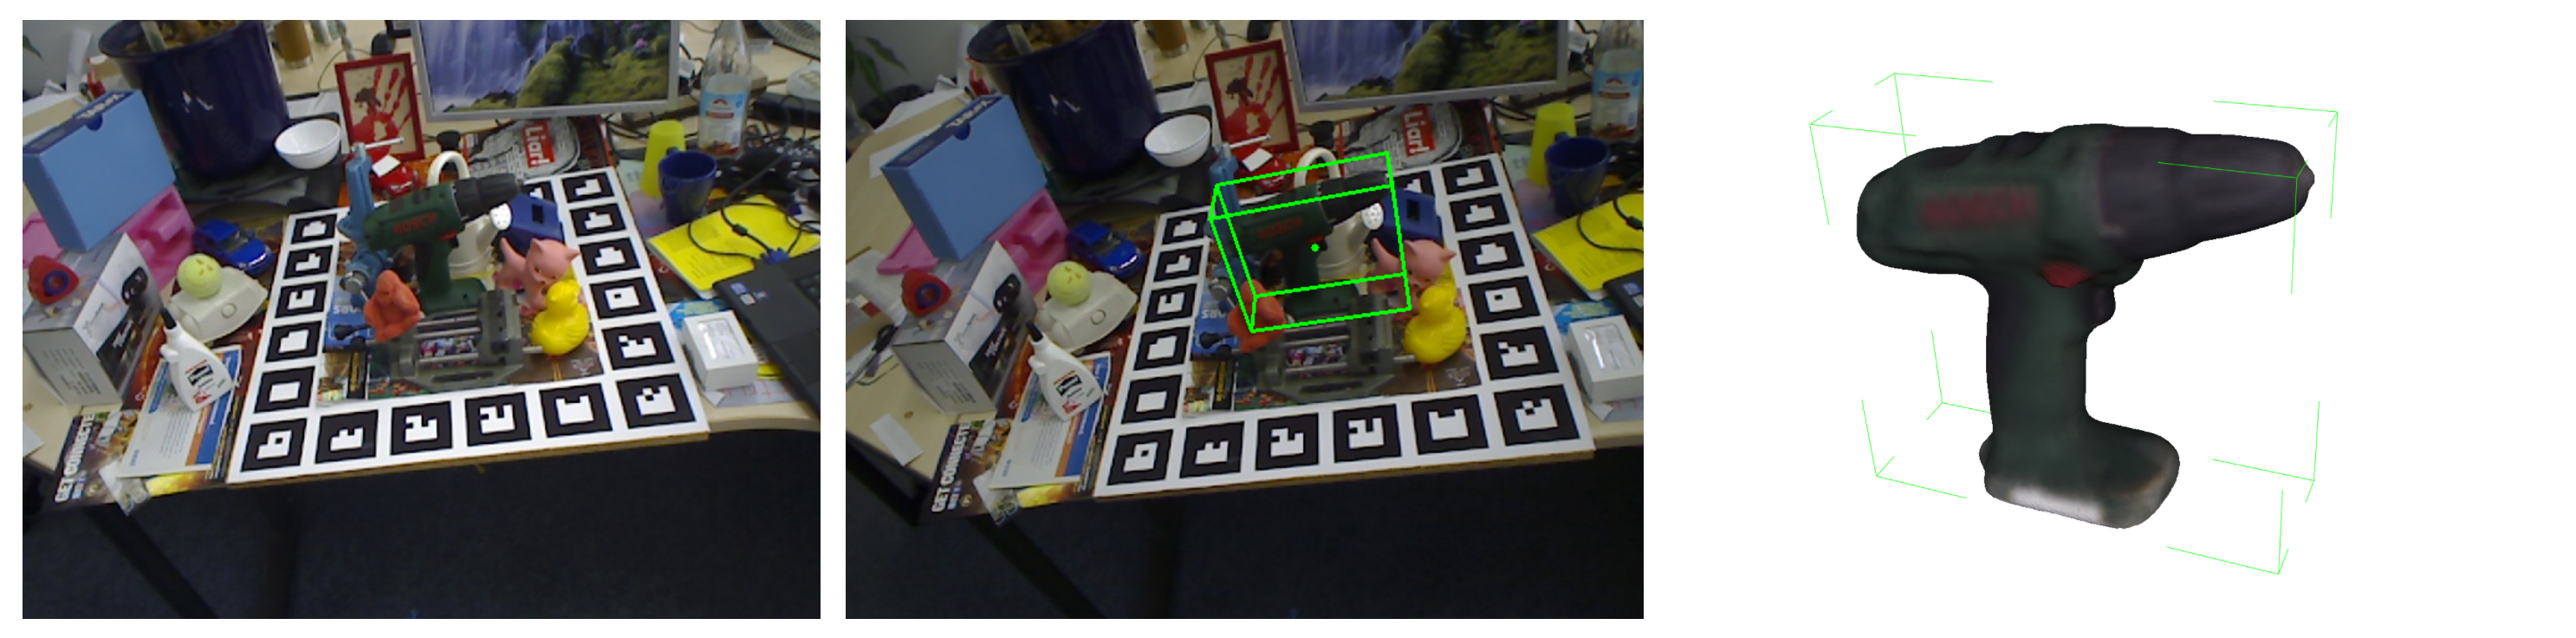
\includegraphics[width=\textwidth]{LINEMOD/LINEMOD.png}
    \caption{A basic overview of the type of data LINEMOD contains: image, ground truth and 3D model and bounding box.}
    \label{fig:linemod}
\end{figure}

The LINEMOD dataset is widely used for training and evaluating 6D pose estimation methods. It is often used as a benchmark to compare different approaches, and is generally the standard we are aiming for.

The dataset contains images and annotations for 13 different objects, placed in 13 different cluttered scenes. For each object, around 1200 images are provided with associated ground truths, including separate rotations and translations. Furthermore, for each object a colored 3D model is provided. The dataset also contains depth images corresponding to each scene, but since our network only takes RGB input, we are not interested in these.

LINEMOD was generated by sticking the tracked objects to the center of a board surrounded by markers. Since the position of each object on the board is known, and the marker pose relative to the camera can be easily and robustly estimated as described in section \ref{s:notlearningbasedmethods}, the final pose of the object can be computed with excellent accuracy. Furthermore, since the images were taken in a uniformly divided hemispherical space around the center board, each object has images comprising a good distribution of poses from multiple orientations.

\subsection{Occlusion LINEMOD}

Occlusion LINEMOD\cite{occlusionlinemod} is a multi-object pose estimation dataset that builds on a subset of LINEMOD; in particual it only uses images from one scene of the 13 provided. It differs from the base dataset in two aspects: first, that all objects are annotated in every scene, and second, that objects often present heavy occlusion due to clutter and positioning. This makes it extremely challenging when compared to vanilla LINEMOD.

Occlusion has been used mainly to train RGB-D models, but some pure RGB approaches \cite{PVNet}\cite{PoseCNN} have also used it as a test dataset, while employing LINEMOD for training. EfficientPose, being a multiple object detection network, employs Occlusion for both training and testing one of its models.

\section{Rendered Datasets}

We find ourselves in the situation where we want to train a 6D pose estimation model on a certain set of objects, that are not present in any available dataset. This necessarily means that we must create our own datasets for training and evaluation.

To create our own datasets we require images with their associated ground truths. However, collecting this data in the real world is tedious and difficult, considering that any errors or biases will affect perfomance of the final model. 

One possible solution is to use rendering software, which can potentially generate infinite quantites of training images. However, while a model trained on this data could certainly work well in simulation, we have no guarantee that it also works with real life images. This is because a simulated sensor and simulated enviroment are unable to reproduce unmodeled physical effects and noise in the same way an optical sensor would. This issue is dubbed the "reality gap"\cite{domainRandomization2}, and there are various ways we could attempt to solve it.

\subsection{Randomized Domain Dataset}

Domain Randomization\cite{domainRandomization} is the most readily available method for bridging the reality gap. The hypothesis behind this concept states that introducing sufficient variability in the simulated training domain will allow the model to generalise to the real world with no additional steps.

In our situation, the domain is an image, so we have a huge variety of ways we could theoretically randomize it. For our first attempt, we decided to generate a dataset for estimating the pose of a single object: a standard M6x30 hexagonal head screw. This is a very challenging object for pose estimation, as it is small (34 mm in length) and symmetric. The reason why symmetric objects are difficult for pose estimation is explained in depth in section (t.b.a.).

To render the images in our dataset, we use Unity's Perception package\cite{unityPerception}, which integrates domain randomization features into its pipeline. Unity Perception works by implementing an object called a scenario, which is connected to a set of scripts called randomizers. When we run a scenario, we specify the number of iterations and the number of frames we want to render for each iteration, and at the beginning of each iteration, all randomizers connected to the scenario are called to set one of the domain variables. These variables can be anything within the scene, from positions and rotations of objects to textures and colors.

\begin{wrapfigure}{r}{0.5\textwidth}
    \centering
    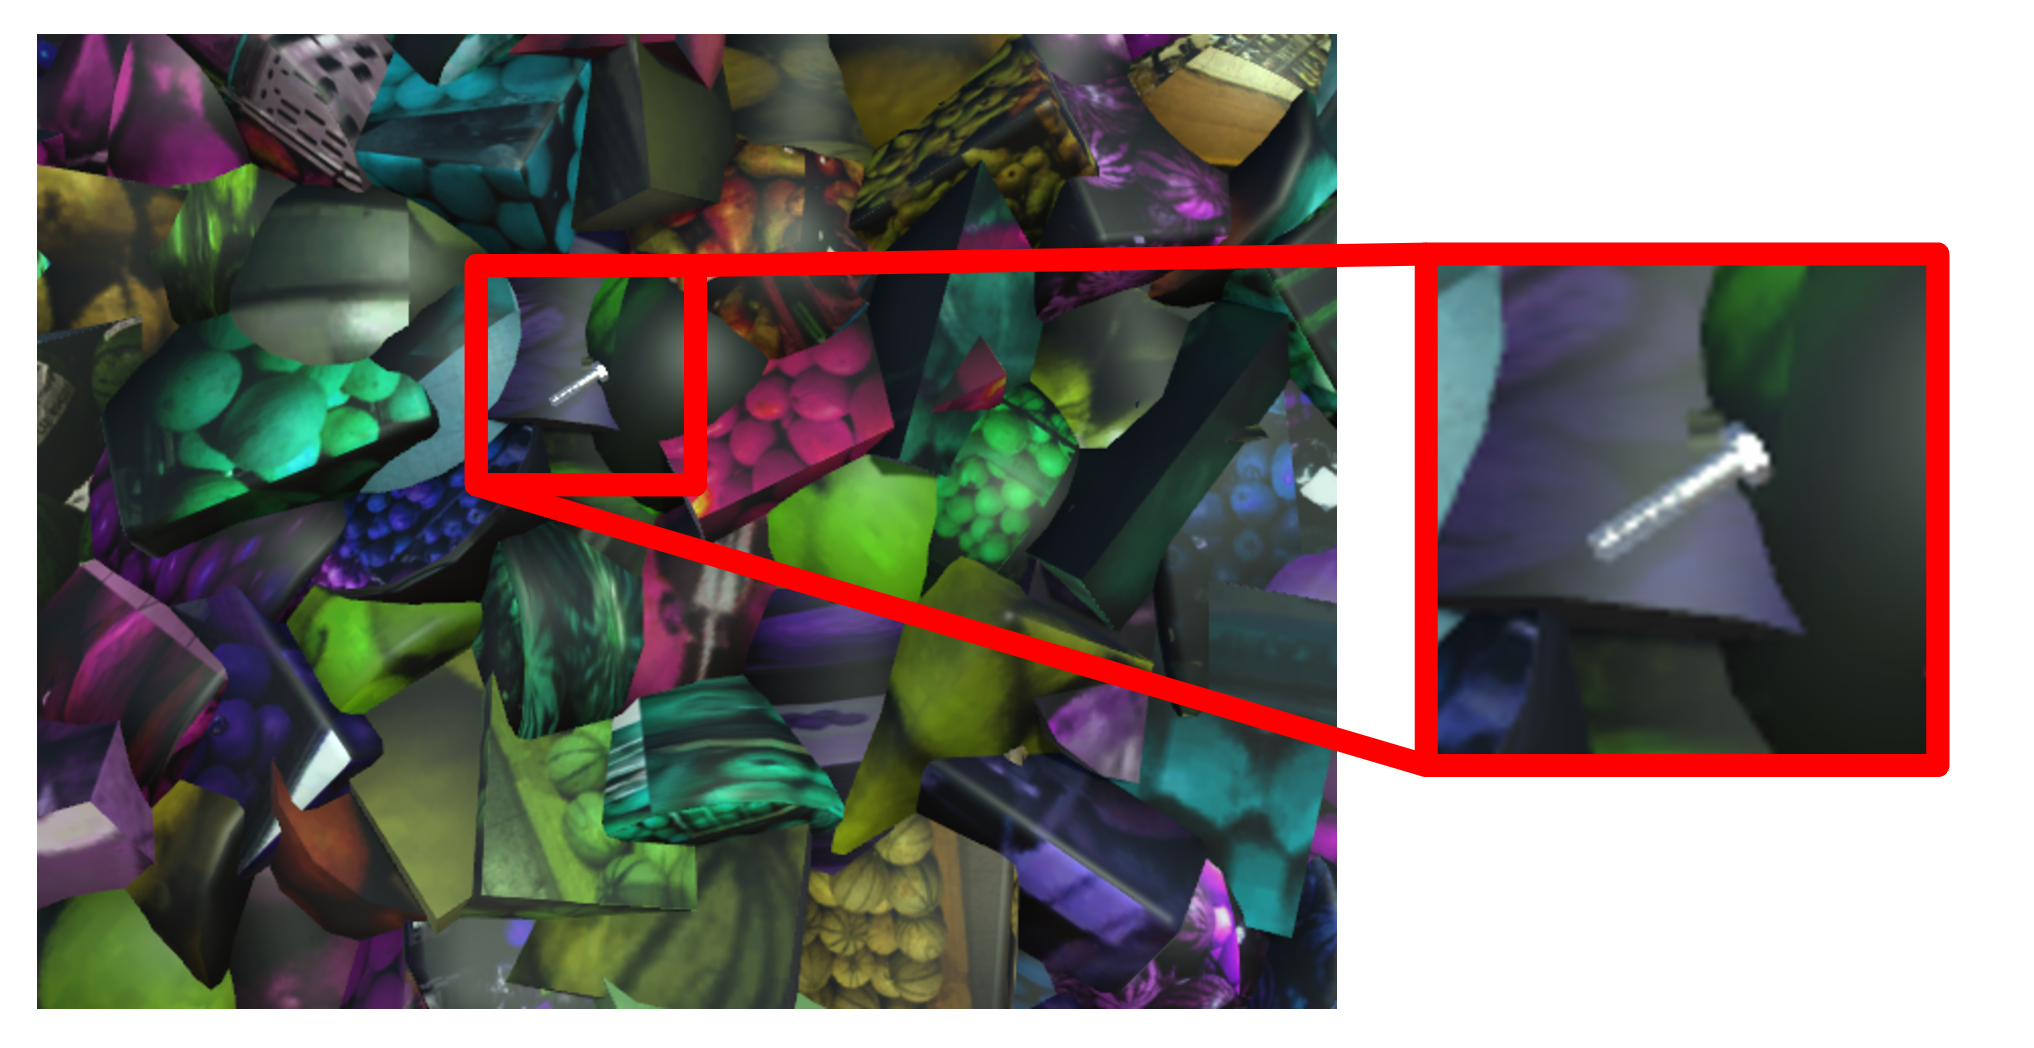
\includegraphics[width=0.5\textwidth]{screwdataset/ScrewDataset.png}
    \caption{A sample of an image generated with Unity's Perception package.}
    \label{fig:screwdataset}
\end{wrapfigure}

For our dataset, we implemented a scenario with 10'000 iterations lasting one frame each. We used a model of the M6x30 screw from the FreeCAD Fasteners workbench\cite{Fasteners}, and then used a custom randomizer to set its position and rotation for each iteration. We then used default randomizers provided as samples by Unity as part of its Perception package to generate a background, composed by random shapes placed in random positions with random orientations and textures. Finally, we used a custom randomizer to set the lighting color, intensity and origin. A sample image from this dataset appears in figure \ref{fig:screwdataset}.

We then converted the Unity output to a format that we could feed to EfficientPose for training. This required converting the ground truths from Unity's internal left-handed reference system to the right-handed reference used by the rest of the world, and generating other relevant information required by EfficientPose, such as the masks for the  